\documentclass{article}
\usepackage{amsmath}
\usepackage{verbatim}
\usepackage[margin=0.5in]{geometry}
\setlength\parindent{0pt}
\usepackage{color}
\usepackage{graphicx}
\usepackage{hyperref}
% \usepackage{subcaption}
%\usepackage{tabularx}
\usepackage{float}

\begin{document}


\begin{center}
\Huge{\textsc{Homework 3}} 

\Large\textsc{CMPS242 - Fall 2015}\\

\large{Ehsan Amid \hfill Andrei Ignat  \hfill Sabina Tomkins} 
\end{center}

\section{Problem 1}

a) After saving the file in an aff file, we run the linear regression algorithm on the data and get the following values for the parameters:

$w = [-0.1343, 1.8477,  -0.8966]^\top$ and $b = 4.3608$ where $\hat{y} = w^\top \mathbf{x} + b$

The root mean squared error on the training set is: $0.1897$\newline

b) The prediction for the new instance $\mathbf{x} = [3, 3, 5]$: $\hat{t} = 5.0180$\newline

c) Now, we set the regularizer $\lambda = 0.2$ and run the first two parts again to get:

$w = [-0.1527, 2.0598, -0.6439]^\top$ and $b = 1.9483$

As can be seen, the weights become smaller, compared to (a), as we expected.

The root mean squared error on the training set becomes: $0.4614$\newline 

d) By doing the calculations by hand, we find the following weights:

$w = [ -0.1343, 1.8477, -0.8966]^\top$ and $b = 4.3608$ and error $= 0.1897$, which is almost the same as part (a), because Weka uses a very small regularizer parameter by default ($1e-8$).\newline

e) The least squared error solution does not depend on the order of the examples because what we are trying to minimize is the sum of the squared errors.\newline

\section{Problem Two}
\subsection{Part a}
Select the Use training set test option and run the three classifiers. Report their results (accuracies). Which algorithm is best and why?

\begin{table}[H]
    \begin{center}
    \caption{Accuracies on training set}
    \begin{tabular}{|c|c|c|c|}
   \hline
        & Nearest Neighbor & Naive Bayes & Logistic Regression \\ \hline
         Accuracy Training Set &  100\%&76.3021\% & 78.2552\%   \\ \hline
         Accuracy 66\% Split &  72.7969 \% &77.0115 \% & 80.0766 \% \\\hline
             
     
    \end{tabular}
    \end{center}
\end{table}

At first glance it may appear that 1 Nearest Neighbor is the best. However it's performance is so nice on the training set that one is agitated by a fear of the model having overfitted the data. Indeed that seems to be the case, when we perform a 66\% split training, testing, we see that the 1 Nearest Neighbor is the least impressive of the lot. 

\subsection{Part b}
From weka we have that the coefficients are: 

\begin{table}[H]
 \caption{Coefficients}
    \begin{center}
    \begin{tabular}{|c|c|c|c|}
   \hline
preg          &       -0.1232\\
plas             &    -0.0352\\
pres               &   0.0133\\
skin              &   -0.0006\\
insu               &   0.0012\\
mass              &   -0.0897\\
pedi             &    -0.9452\\
age            &      -0.0149\\
Intercept      &       8.4047\\ %bias
\hline
    \end{tabular}
    \end{center}
\end{table}

We chose point 643, and got the result was -0.004295 Which we confirm is close to 0. Rerunning a sanity chance of P(x) = 1/(1+$e^x$) = .5. 

\subsection{Part c}
\begin{table}[H]
    \begin{center}
     \caption{Accuracies with 10-Fold Cross validation}
    \begin{tabular}{|c|c|c|c|}
   \hline
        & Nearest Neighbor & Naive Bayes & Logistic Regression \\ \hline
         Accuracy 10 Fold Cross Validation &  70.1823\%&76.3021\% &  77.2135 \%   \\ \hline
       
             
     
    \end{tabular}
    \end{center}
\end{table}

We see that the accuracy for Naive Bayes remains the same. The accuracy for Nearest Neighbor is greatly decreased. The accuracy for logistic regression suffers only slightly. Thus we see that Naive Bayes and Logistic Regression are more robust algorithms. 

\subsection{Part d}
Use preprocessing to normalize the features (use the preprocess tab and select unsupervised, attribute, normalize). Read the information on this method, and look at the new attribute values. What did it do?

It fit a normal distribution to each feature, finding the mean, standard deviation, count, and precision for each class and each feature. That is each attribute is transformed as follows: 
\begin{center}
Let $x_i$ be an instance from feature class $i$. \\
$x_i' = (x_i-\mu_i)/\sigma_i$
\end{center}

Rerun the logistic regression with 10-fold cross validation and the attributes normalized. Did the accuracies change? Why?

The accuracies did not change. It won't change because normalizing is applying a linear transformation to all features so this may rescale or shift the decision boundary, and the points, but all with respect to each other so the actual decisions will not change, and the accuracy will remain the same. 

The coefficients changed but not by that much. 
\begin{table}[H]
    \begin{center}
     \caption{Coefficients after normalizing}
    \begin{tabular}{|c|c|c|c|}
   \hline
preg          &        -2.0941\\
plas             &    -6.9976\\
pres               &    1.6221\\
skin              &  -0.0613\\
insu               &   1.0082\\
mass              &    -6.0189\\
pedi             &    -2.2136\\
age            &       -0.8921\\
Intercept      &        8.0187\\ %bias
\hline
    \end{tabular}
    \end{center}
\end{table}

There are dramatic changes to the weight vector. Each weight grew by several orders of magnitude. 

\subsection{Part e}
In logistic regression, the ridge parameter penalizes large weights. What happens to the cross validation accuracy and hypothesis weights when it is set to 0? How about when it is increased (to say 0.3)?

The cross validation does not change when it is set to zero, the default value of 1.0$10^{-8}$ is already quite small. The accuracy improves slightly with a larger ridge parameter of 3, to 77.6, but it does not change at .30. 

The hypothesis weights do not change much. In this case we did not normalize the features. 

\begin{table}[H]
    \begin{center}
    \caption{Ridge Paramter .3}
    \begin{tabular}{|c|c|c|c|}
   \hline
preg          &        -0.1221\\
plas             &     -0.0349\\
pres               &    0.0131\\
skin              &   -0.0006\\
insu               &    0.0012\\
mass              &    -0.0889\\
pedi             &     -0.9376\\
age            &        -0.015\\
Intercept      &        8.3495\\ %bias
\hline
    \end{tabular}
    \end{center}
\end{table}

\begin{table}[H]
    \begin{center}
    \caption{Ridge Paramter 0.0}
    \begin{tabular}{|c|c|c|c|}
   \hline
preg          &       -0.1232\\
plas             &      -0.0352\\
pres               &    0.0133\\
skin              &   -0.0006\\
insu               &    0.0012\\
mass              &     -0.0897\\
pedi             &     -0.9452\\
age            &        -0.0149\\
Intercept      &        8.4047\\ %bias
\hline
    \end{tabular}
    \end{center}
\end{table}


\subsection{Part f}
Would you expect 3NN or 5NN do better than Nearest Neighbor? Why? Test your hypothesis by using IBk in the lazy folder and report the resulting accuracies.

Yes, we would. The model is more complex so it should obtain better results as long it does not overfit. 


\begin{table}[H]
    \begin{center}
    \caption{K Nearest Neighbor Results}
    \begin{tabular}{|c|c|c|c|}
   \hline
        & 1 Nearest Neighbor & 3 Nearest Neighbor  & 5 Nearest Neighbor  \\ \hline
         Accuracy 10 Fold Cross Validation &  70.1823\%&72.6563\% &  73.1771 \%   \\ \hline
       
             
     
    \end{tabular}
    \end{center}
\end{table}

\subsection{Part g}
Create a modified version of the diabetes dataset by picking one attribute at random and adding 10 additional copies of that attribute to the data set (or.are). There should be the same number of examples, but each example will now have 19 rather than 9 attributes (including the class label). How would you expect the 10-fold cross validation accuracies of the classifiers to change? Run the classifiers on the modified .arff fille and report the changes.

We do not expect to see changes in the accuracy as we are applying the same noise to each data point. However the accuracy of the Naive Bayes and 1 Nearest Neighbor do go down slightly. 

The results are shown in table 5. 


\begin{table}[H]
    \begin{center}
    \caption{Adding 10 attributes}
    \begin{tabular}{|c|c|c|c|}
   \hline
        & Nearest Neighbor & Naive Bayes & Logistic Regression \\ \hline
         Accuracy 10 Fold Cross Validation &  70.7031\%&67.5781\% &  77.2135 \%  \\ \hline
        \end{tabular}
    \end{center}
\end{table}

\subsection{Part h}
Please see table 6. We see again that the accuracy of logistic regression stays the same. However the accuracy of the nearest neighbor went down significantly. 

\begin{table}[H]
    \begin{center}
    \caption{Adding random noise}
    \begin{tabular}{|c|c|c|c|}
   \hline
        & Nearest Neighbor & Naive Bayes & Logistic Regression \\ \hline
         Accuracy 10 Fold Cross Validation &  57.1615\%&76.3021\% &  77.2135 \%  \\ \hline
        \end{tabular}
    \end{center}
\end{table}

\section{Problem 3}

\paragraph{a)}
After running the code, we see that the perceptron manages to finish after $2$ epochs with an average of approximately 10 errors in the first epoch(and no errors in the second epoch). We note that, due to the setup of the labels, what the perceptron is doing in this part of the problem is to just learn that it should always predict with the label of the first feature. In other words, the weight vector $\mathbf{w}$ that will always have a large value for the first feature i.e.

\[
\mathbf{w}_1 >> \mathbf{w}_{2,\hdots,15} 
\]

\paragraph{b)}
In the second part of the problem, the label is affected by all of the features in the dataset. In other words, the label is now the result of a non-linear mixture of the features of each vector. Since the perceptron is built in such a way that it should predict the \textit{linear dependence} of different features of the datapoints, we immediately realize that the perceptron will never manage to learn a weight vector $\mathbf{w}$ such that it yields no errors whatsoever. In Figure~\ref{fig:prcp}, one can see that throughout 1000 epochs, the error count of the perceptron follows two trends: firstly, the error count is stable in the sense that it always lies in a closed interval and secondly, there is a repetitive pattern to the error fluctuation. Since our learning rate $\eta_i=1$ is constant, training the perceptron will never converge to an error count of 0.

\begin{figure}[H]
\centering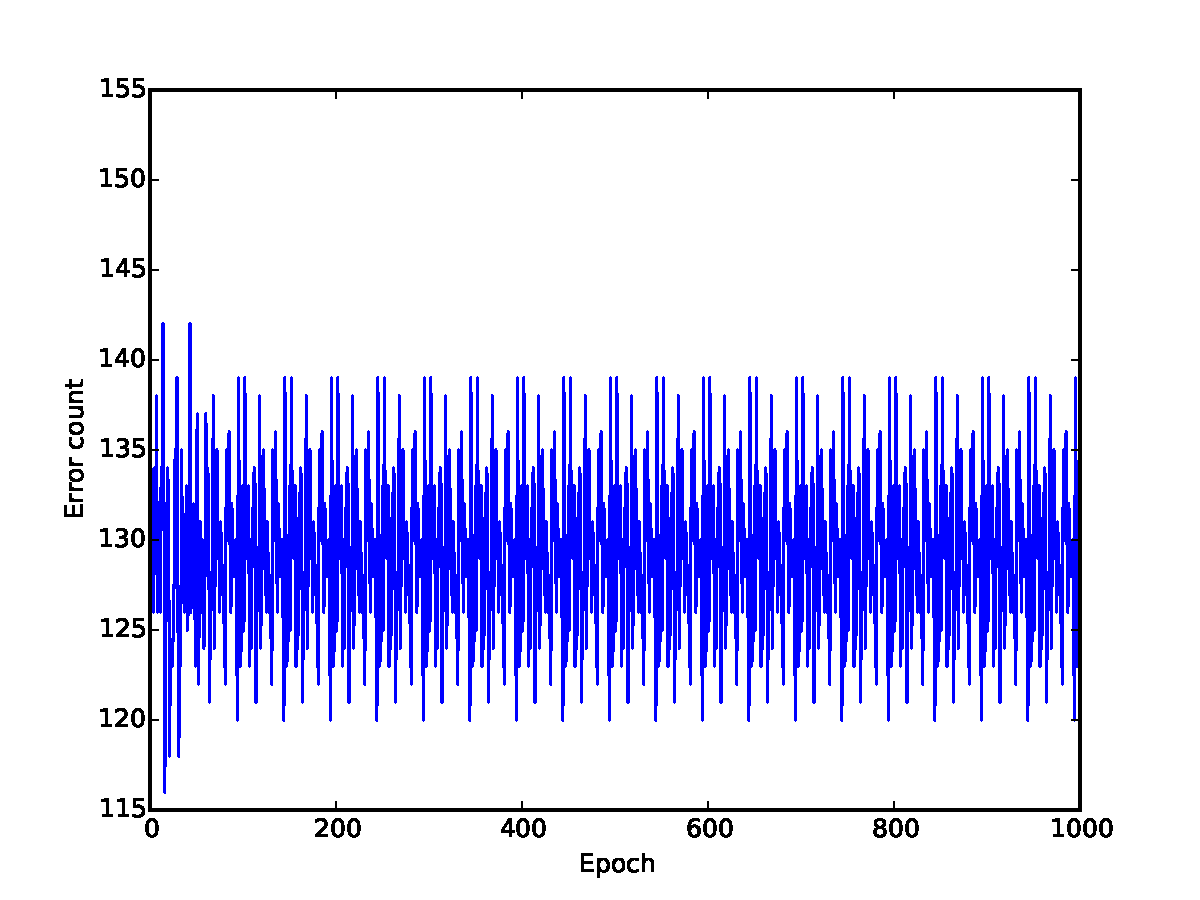
\includegraphics[width=0.5\textwidth]{prcp.pdf}
\caption{Perceptron error rate over 1000 epochs}\label{fig:prcp}
\hfill
\end{figure}

\paragraph{c)}
The following table contains the averages over 10 different test sets for the hypothesis described in part c).

\begin{table}[H]
    \begin{center}
    \begin{tabular}{c|c|c|c|c}

		Last hypothesis & Average hypothesis & Voted hypothesis & Last epoch average & Last epoch vote \\
	   \hline		125.8 & 125.8 & 125.8 & 125.8 & 125.8
        \end{tabular}\caption{Average error count over 10 different test sets}
    \end{center}
\end{table}

At first, it might look like there is a typo in our table. That is however not the case. Comparing to the labeling executed in part \textbf{b)}, we see that part \textbf{c)} has the same non-linearities in the labeling procedure. This means that, regardless of the number of epochs, the perceptron cannot determine an accurate weight vector $\mathbf{w}$ simply because this vector does not exist. Therefore, we will never reach an error count of 0. Now, why are all the average error counts the same?
In the \textit{last hypothesis} case, one simply uses the most recent weight vector. This weight vector contains all the information that the previous weight vectors contained and as such, it is to be expected that using this hypothesis, we would get the same error count as in the case of the \textit{average hypothesis} case and the \textit{voted hypothesis} case. In these two cases, we again consider all the weight vectors, either under the form of a voting scheme or under the form of an average weight vector. While \textit{last epoch average} and \textit{last epoch vote} only consider weight vectors from the last epoch, these weight vectors contain the same information as the other cases and as such, all of the five hypothesis are, on average, completely equivalent to one another(it might happen that random fluctuations in the test set throw off the error count in specific cases, but on average, the five cases will have the same accuracy).

Since the five hypothesis are equivalent to one another, we expect that their accuracy should be the same. That being said, an example of a non-equivalent hypothesis class would be one that considers e.g. only the first 10 weight vectors. This then would mean that the rest of the information from the learning phase is lost and hence this would yield a different accuracy than the five hypothesis presented in \textbf{c)}.
\section{Problem 4}

Note that

\begin{equation*}
\frac{d \sigma(a)}{d a} = \frac{\exp(-a)}{(1+ \exp(-a))^2} = \sigma(-a) (1-\sigma(-a))
\end{equation*}
and
\begin{equation*}
\frac{d y_n}{d \mathbf{w}} = \sigma(-a) (1-\sigma(-a)) \mathbf{x}_n = y_n (1-y_n) \mathbf{x}_n
\end{equation*}
Taking the derivative of $E(\mathbf{w})$ w.r.t. $\mathbf{w}$ and substituting for these $\frac{d y_n}{d \mathbf{w}}$ from above, we have:
\begin{equation*}
\nabla E(\mathbf{w}) = \sum_{n=1}^N (\frac{t_n}{y_n}  - \frac{(1-t_n)}{(1-y_n)}) \frac{d y_n}{d \mathbf{w}} = \sum_{n=1}^N (t_n(1-y_n)-(1-t_n)y_n) \mathbf{x}_n = \sum_{n=1}^N(t_n - y_n)\mathbf{x}_n
\end{equation*} 

\end{document}
